% ********** Chapter 4 **********
\chapter{Solution}
\label{sec:Solution}

There are two kind of connection solution of the core of Web Call, the Relay Call and Third Party Call. The different between them is the way they handle media stream.

The Relay Call Controller works as a back-to-back agent and forwards media streams, while Third Party Call Controller only establishes connections by sending out SIP messages and it does not handles any streams itself. 

\section{Relay Call}
\label{sec:Solution:RelayCall}

\begin{figure}[!hbtp]
\centering
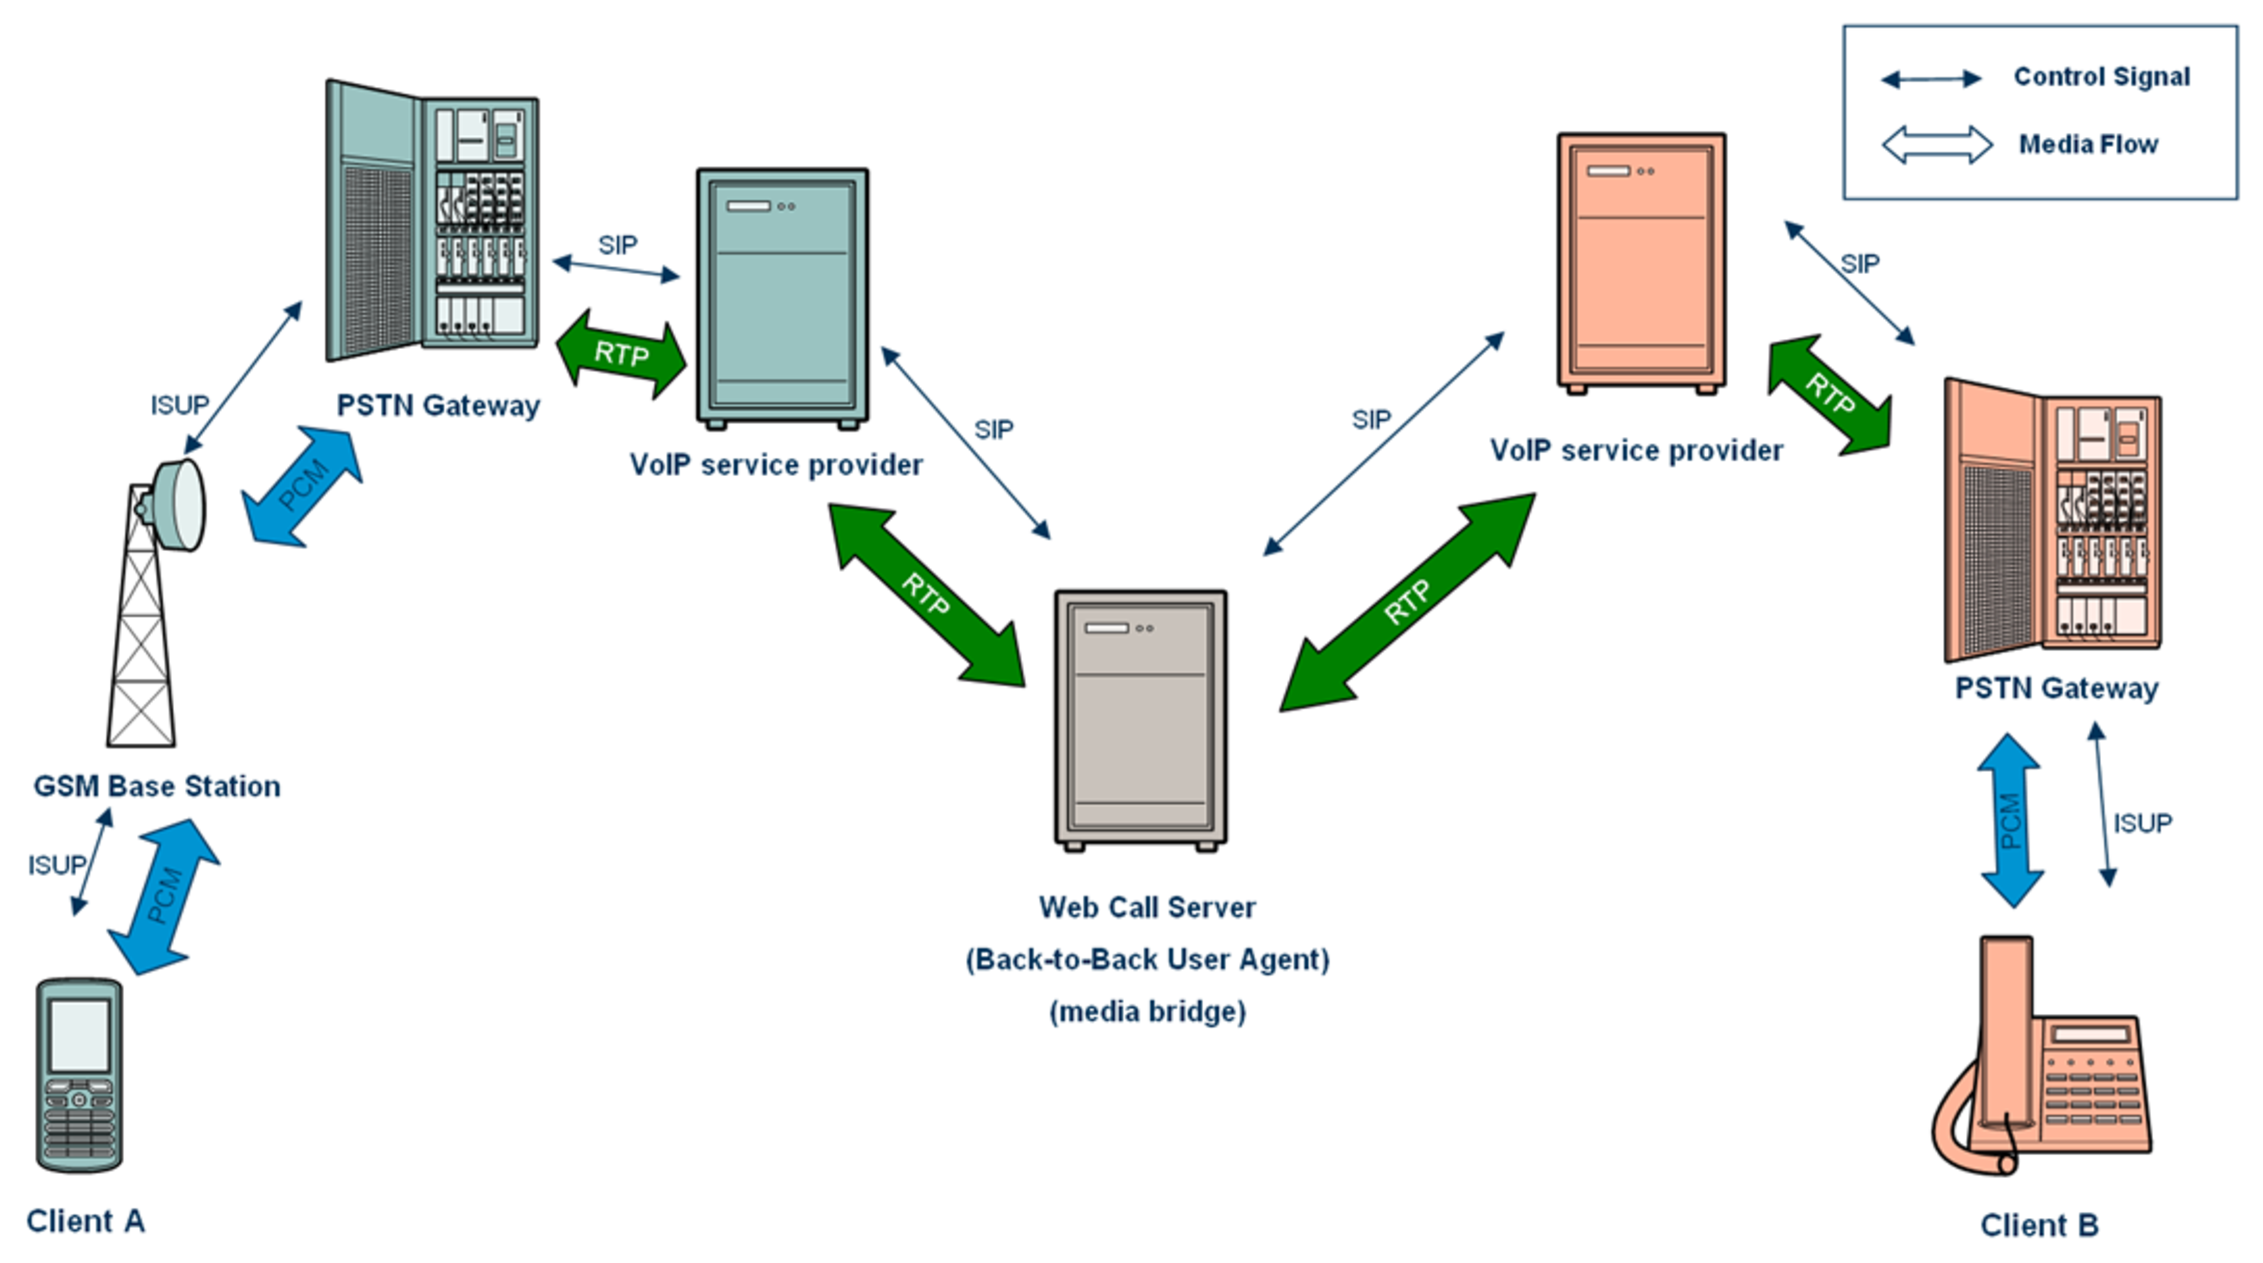
\epsfig{file=chap04/resources/the_signal_and_media_flow_of_relay_call, width=5.34in}
\caption{The signal and media flow of Relay Call}
\label{fig:TheSignalAndMediaFlowOfRelayCall}
\end{figure}

The signal and media flow of Relay Call is shown in Figure \ref{fig:TheSignalAndMediaFlowOfRelayCall}. In this scenario, the Web Call Example Application acts as a back-to-back user agent. It sets up the connection and forwards the media stream. It can be seen from the picture that both signal and media are handled by Web Call Server. When it starts, it try to call client A. After it establishes a session with client A, it will try to call client B and also establish a session with client B. After that, it will work as a media stream bridge and forward media stream from client A to B, as well as from client B to A.



\section{Third Party Call}
\label{sec:Solution:ThirdPartyCall}

In the traditional telephony context, third party call control allows one entity (which we call the controller) to set up and manage a communications relationship between two or more other parties. Third Party call control (referred as 3pcc) is often used for operator services (where an operator creates a call that connects two participants together) and for conferencing. The signal and media flow in third party call is show in Figure \ref{fig:TheSignalAndMediaFlowOf3pc} The advantage of third party call in Web Call is that the controller only need to handle message transfer and leaves the media flow for the ISP.

\begin{figure}[!hbtp]
\centering
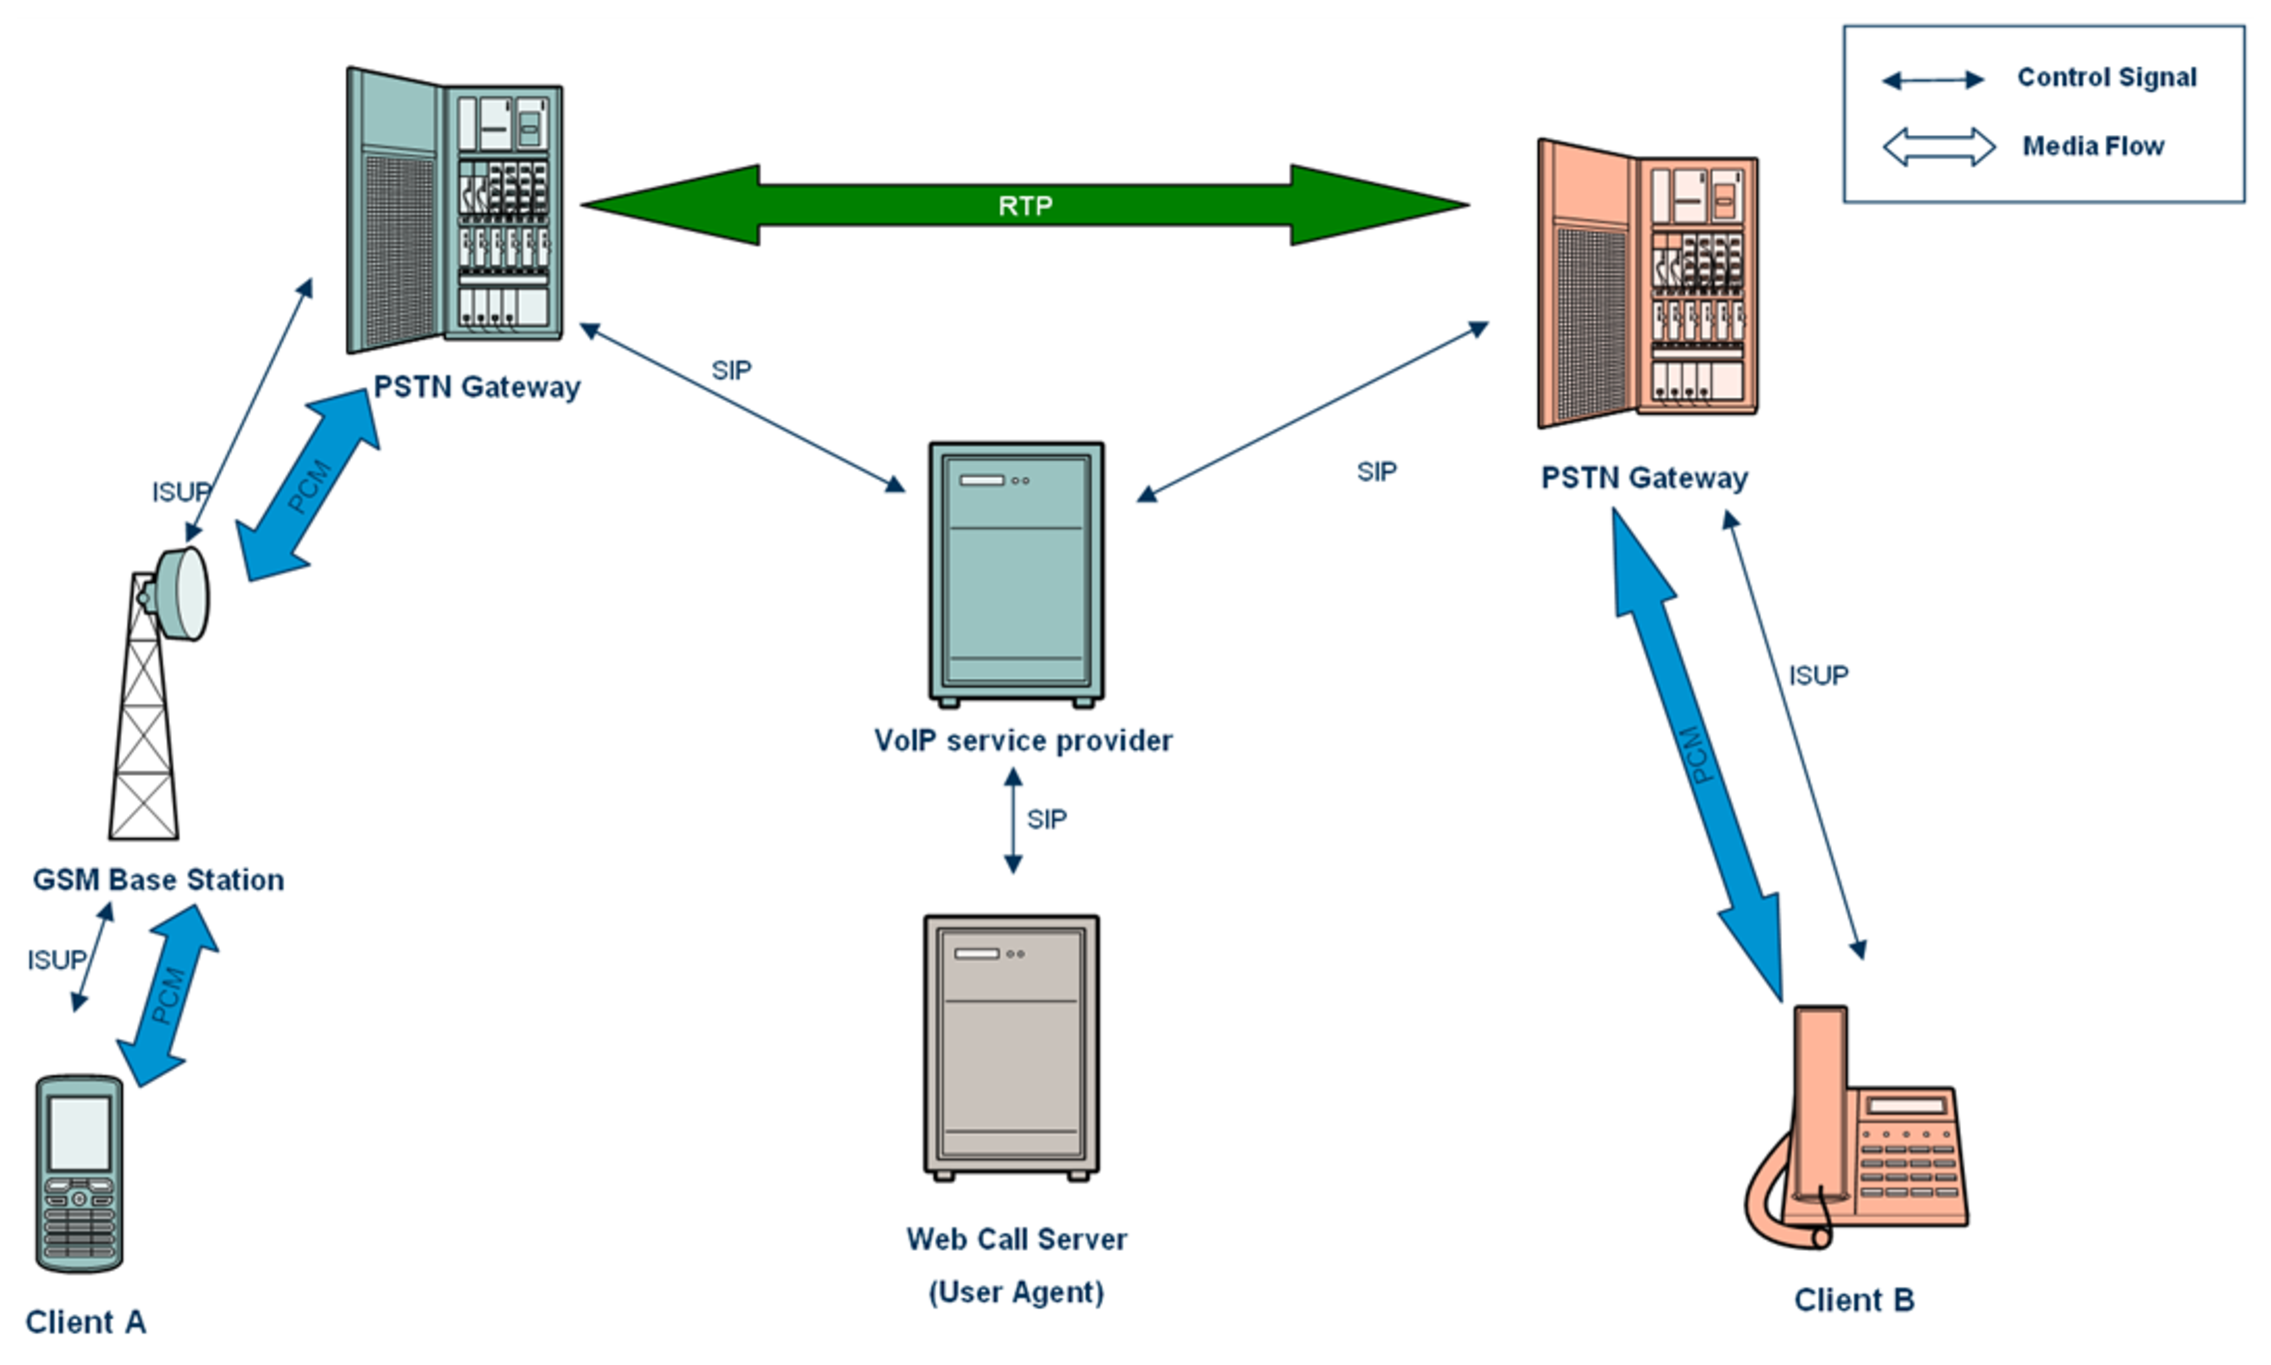
\epsfig{file=chap04/resources/the_signal_and_media_flow_of_3pc, width=5.34in}
\caption{The signal and media flow of Third Party Call}
\label{fig:TheSignalAndMediaFlowOf3pc}
\end{figure}




\subsection{Call Transfer}
\label{sec:Solution:ThirdPartyCall:CallTransfer}


\subsection{SDP Swap}
\label{sec:Solution:ThirdPartyCall:SDPSwep}

\subsection{Re-invite}
\label{sec:Solution:ThirdPartyCall:Re-invite}

\subsection{Web Client}
\label{sec:Solution:ThirdPartyCall:WebClient}


\section{Conclusion}
\label{sec:Solution:Conclusion}




% ********** End of chapter **********
